% generated by scripts/pkl_to_latex.py
% source PKL : thermal_v1_L8_Ne8_U10_t1_mode-uniform_tpall_t2all_tperpall_nmin2_solver-gcg_full_restarts8_iter200_kmax4_tol1em09_cut10_adaptive1_step5_clusteravg1_T0to0.5_N20-3c87501b406b_knone_diag0.pkl
% scan type  : Tscan
% state      : gs
% quantity   : linear-entropy
% x-max cap  : 0.3 (cut at k_B T/t = 0.3, supervisor 4 Nov 2026)
% requires   : \usepackage{pgfplots} \pgfplotsset{compat=1.18}
% colours match the matplotlib PDF (tab10 cycle)
\definecolor{gmeC0}{HTML}{1F77B4}
\definecolor{gmeC1}{HTML}{FF7F0E}
\definecolor{gmeC2}{HTML}{2CA02C}
\definecolor{gmeC3}{HTML}{D62728}
\definecolor{gmeC4}{HTML}{9467BD}
\definecolor{gmeC5}{HTML}{8C564B}
\definecolor{gmeC6}{HTML}{E377C2}
\definecolor{gmeC7}{HTML}{17BECF}

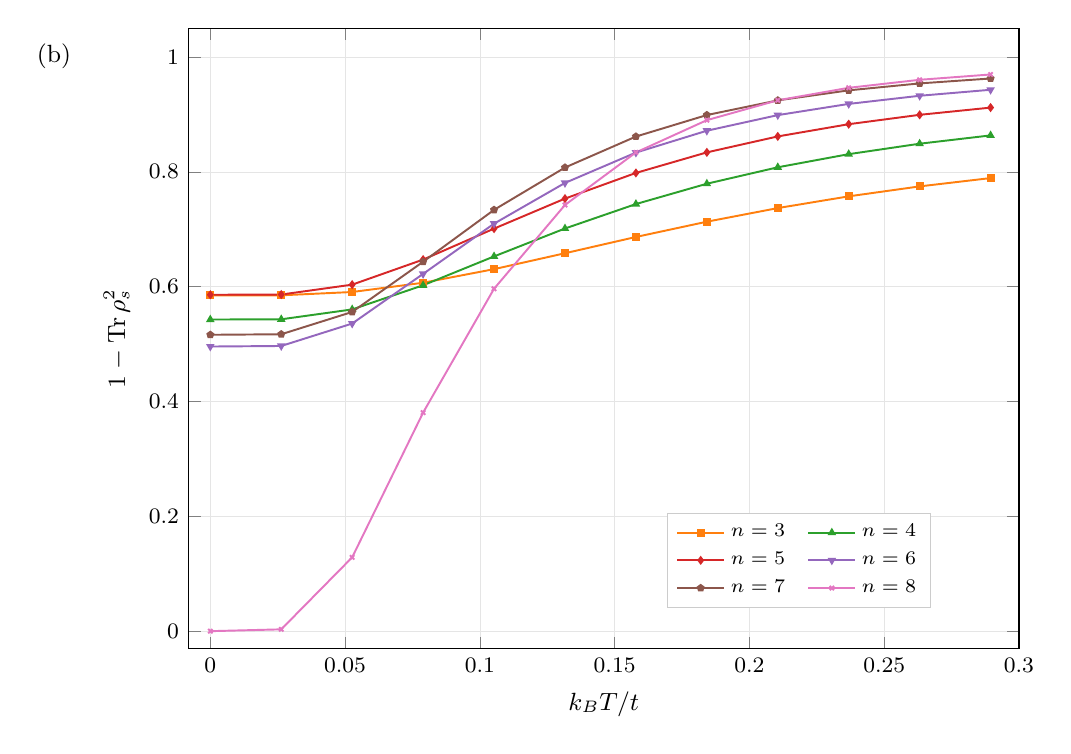
\begin{tikzpicture}
  \begin{axis}[
    width=\columnwidth,
    height=0.78\columnwidth,
    xlabel={$k_B T/t$},
    ylabel={$1-\mathrm{Tr}\,\rho_s^2$},
    grid=both,
    grid style={line width=.1pt, draw=gray!20},
    tick label style={font=\footnotesize\rmfamily, /pgf/number format/fixed},
    label style={font=\small\rmfamily},
    scaled ticks=false,
    legend style={font=\scriptsize\rmfamily, draw=gray!40, at={(0.5,1.03)}, anchor=south, /tikz/every even column/.append style={column sep=6pt}},
    legend cell align={left},
    legend columns=2,
    ymin=-0.03,
    ymax=1.05,
    xmin=-0.008,
    xmax=0.3,
    xtick={0,0.05,0.1,0.15,0.2,0.25,0.3},
    legend style={at={(0.735,0.142)}, anchor=center, fill=white},
    after end axis/.append code={\node[anchor=east, font=\small\rmfamily] at (axis description cs:-0.13,0.954) {(b)};},
  ]
    \addplot[color=gmeC1, mark=square*, mark size=1.1pt, line width=0.7pt] coordinates {
        (0,0.584753) (0.026316,0.584886) (0.052632,0.590625) (0.078947,0.606743)
        (0.105263,0.630433) (0.131579,0.658151) (0.157895,0.686471) (0.184211,0.713069)
        (0.210526,0.736779) (0.236842,0.757238) (0.263158,0.774549) (0.289474,0.789037)
    };
    \addlegendentry{$n=3$}
    \addplot[color=gmeC2, mark=triangle*, mark size=1.1pt, line width=0.7pt] coordinates {
        (0,0.542696) (0.026316,0.543109) (0.052632,0.560309) (0.078947,0.602365)
        (0.105263,0.652614) (0.131579,0.701214) (0.157895,0.743793) (0.184211,0.779188)
        (0.210526,0.807821) (0.236842,0.830688) (0.263158,0.848873) (0.289474,0.863351)
    };
    \addlegendentry{$n=4$}
    \addplot[color=gmeC3, mark=diamond*, mark size=1.1pt, line width=0.7pt] coordinates {
        (0,0.585809) (0.026316,0.586218) (0.052632,0.603436) (0.078947,0.647066)
        (0.105263,0.700999) (0.131579,0.753282) (0.157895,0.797989) (0.184211,0.833787)
        (0.210526,0.861571) (0.236842,0.882876) (0.263158,0.899192) (0.289474,0.911748)
    };
    \addlegendentry{$n=5$}
    \addplot[color=gmeC4, mark=triangle*, mark size=1.1pt, mark options={rotate=180}, line width=0.7pt] coordinates {
        (0,0.495677) (0.026316,0.49664) (0.052632,0.535687) (0.078947,0.622158)
        (0.105263,0.709652) (0.131579,0.780589) (0.157895,0.833432) (0.184211,0.871492)
        (0.210526,0.89868) (0.236842,0.918196) (0.263158,0.932365) (0.289474,0.942801)
    };
    \addlegendentry{$n=6$}
    \addplot[color=gmeC5, mark=pentagon*, mark size=1.1pt, line width=0.7pt] coordinates {
        (0,0.516106) (0.026316,0.517059) (0.052632,0.555891) (0.078947,0.64331)
        (0.105263,0.733683) (0.131579,0.8074) (0.157895,0.861346) (0.184211,0.898803)
        (0.210526,0.924344) (0.236842,0.941803) (0.263158,0.953899) (0.289474,0.96244)
    };
    \addlegendentry{$n=7$}
    \addplot[color=gmeC6, mark=x, mark size=1.1pt, line width=0.7pt] coordinates {
        (0,0) (0.026316,0.003173) (0.052632,0.128578) (0.078947,0.380603)
        (0.105263,0.596295) (0.131579,0.742152) (0.157895,0.833695) (0.184211,0.88989)
        (0.210526,0.924507) (0.236842,0.946218) (0.263158,0.960187) (0.289474,0.969441)
    };
    \addlegendentry{$n=8$}
  \end{axis}
\end{tikzpicture}
